% !TeX root = ../index.tex
\documentclass[../index.tex]{subfiles}

\begin{document}
    \section{Wykład 6} 
        \subsection{Wnętrze gwiazdy}
            \subsubsection{Ciśnienie, temperatura, gęstość}
                Wnętrze gwiazdy zaczyna się u podstawy fotosfery \--- miejsca gdzie ośrodek staje się nieprzezroczysty dla promieniowania. Do tego punktu światło dociera z wnętrza poprzez wielokrotne procesy absorbcji i emisji. O warunkach panujących we wnętrzu gwiazdy można dowiedzieć się na podstawie ogólnych praw opisujących budowę gwiazdy. Jednym z nich jest \textbf{równanie równowagi termodynamicznej} \--- w każdym punkcie gwiazdy ciśnienie (głównie termiczne) i siła grawitacji równoważą się:
                \begin{equation}
                    \frac{dp}{dr} = -\rho g
                \end{equation}
                gdzie \(\rho\) \--- gęstość, \(p\) \--- ciśnienie a \(g = G \frac{M_r}{r^2 } \) to przyspieszenie grawitacyjne. Powyższe wyrażenie jest prawidłowe przy założeniu idealnej kulistości gwiazdy. Wszystkie parametry zmieniają się wraz z \(r\). Gdyby gwiazdy nie podlegały równowadze hydrodynamicznej to wówczas zapadałyby się w bardzo krótkim czasie (dynamiczna skala czasowa ewolucji gwiazdy):
                \begin{equation}
                    t_\text{dyn} = \sqrt{\frac{2}{G}} R^{1.5}M^{-0.5} 
                \end{equation}
                Dla słońca \(t_\text{dyn}\) wynosi około pół godziny. Na podstawie równania równowagi termodynamicznej można oszacować ciśnienie wewnątrz słońca. Zmieniając różniczkę na różnice ciśnień na powierzchni i wewnątrz gwiazdy oraz wstawiając po prawej stronie uśrednioną gęstość i przyspieszenie grawitacyjne na panujące na powierzchni słońca otrzymuje się wzór:
                \begin{equation}
                    p_c \sim \frac{GM^2 }{\frac{4}{3}\pi R^{4}} \sim 10^{15}\: Pa \label{eq:star_pressure}
                \end{equation}
                Otrzymany wynik jest ponad dwudziestokrotnie niższy od rzeczywistego, ale daje pojęcie o rzędzie wielkości. W podobny sposób, korzystając z \textbf{równania gazu doskonałego}:
                \begin{equation}
                    p = \frac{k_B}{\mu m_u} \rho T
                \end{equation}
                gdzie \(\mu\) \--- średni ciężar cząsteczkowy w atomowych jednostkach masy. Po przekształceniu wzoru i wykorzystaniu wzoru \ref{eq:star_pressure} otrzymuje się:
                \begin{equation}
                    T_c = \mu_c \frac{m_u}{k_B} G \frac{M}{R} = 1.9 \cdot 10^{7}\: K
                \end{equation}
                Powyższy wynik jest znów zawyżony o \(3.5 \cdot 10^{6}\: K\). Idąc dalej można wyznaczyć gęstość \(\rho_c = 60000\: \frac{kg}{m^3 }\) i to ponownie \(2.5\) raza zaniżony wynik względem dokładniejszych modeli.
            \subsubsection{Źródło energii}
                Źródłem energii gwiazdy jest fuzja termojądrowa zachodzące w jego wnętrzu. Można by się spodziewać, że tak ekstremalne warunki jak wyliczone powyżej pozwalają pokonać siły odpychające od siebie cząstki i łączenie się ich (synteza jądrowa). Energia wydzielona w takim procesie związana jest z \textbf{defektem masy} \--- różnicą pomiędzy masą produktów i substratów (ta różnica to właśnie energia syntezy). Synteza zachodzi dla jąder lekkich (lżejszych niż żelazo). Energia potrzebna do zbliżenia do siebie dwóch protonów to \(1\: MeV\), natomiast w temperaturze \(15\: MK\) średnia temperatura (rozkład Maxwella\--Boltzmanna) wynosi \(1\: keV\). Zgodnie z tym samym rozkładem cząstek praktycznie nie ma w słońcu cząstek, które przekraczają megaelektronowolt. Jednak protonu, jako obiekty kwantowe, mogą przez barierę oddziaływania elektrostatycznego tunelować. Największe znaczenie w fuzji jądrowej mają protony z takiego przedziału energii, że rozkład Maxwella\--Boltzmanna i rozkład prawdopodobieństwa przetunelowania splatają się
                \begin{center}
                    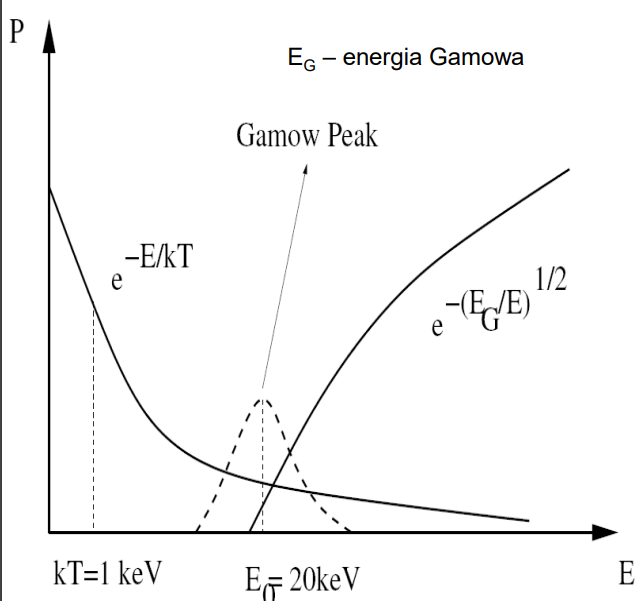
\includegraphics[width=12cm]{images/pikGamowa.png}  
                \end{center}
                Obszar ten nosi miano \textbf{piku Gamowa}.\\
                Do powstania jądra helu potrzeba czterech protonów, lecz jest bardzo mało prawdopodobne, żeby cztery protony z piku Gamowa jednocześnie się zetknęły. Jednak zachodzą reakcje pośrednie. Rozróżniamy dwa możliwe łańcuchy reakcji \(pp\)(proton\-proton) i \textbf{CNO} (węglowo-azotowo-tlenowy):
                \begin{center}
                    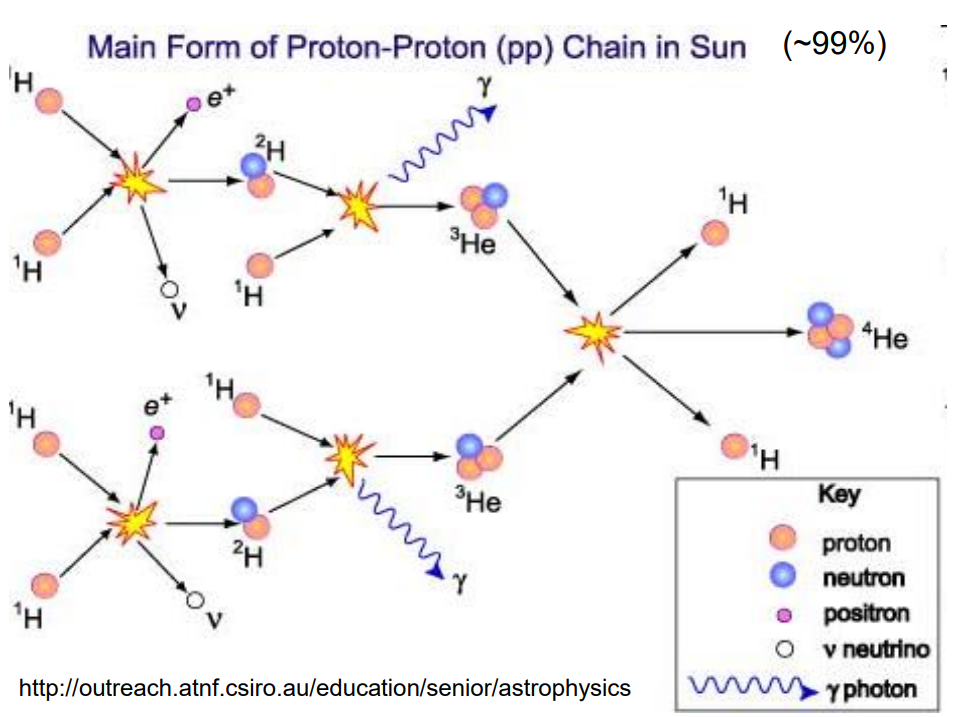
\includegraphics[width=15cm]{images/ppSynteza.png}
                \end{center}
                \begin{center}
                    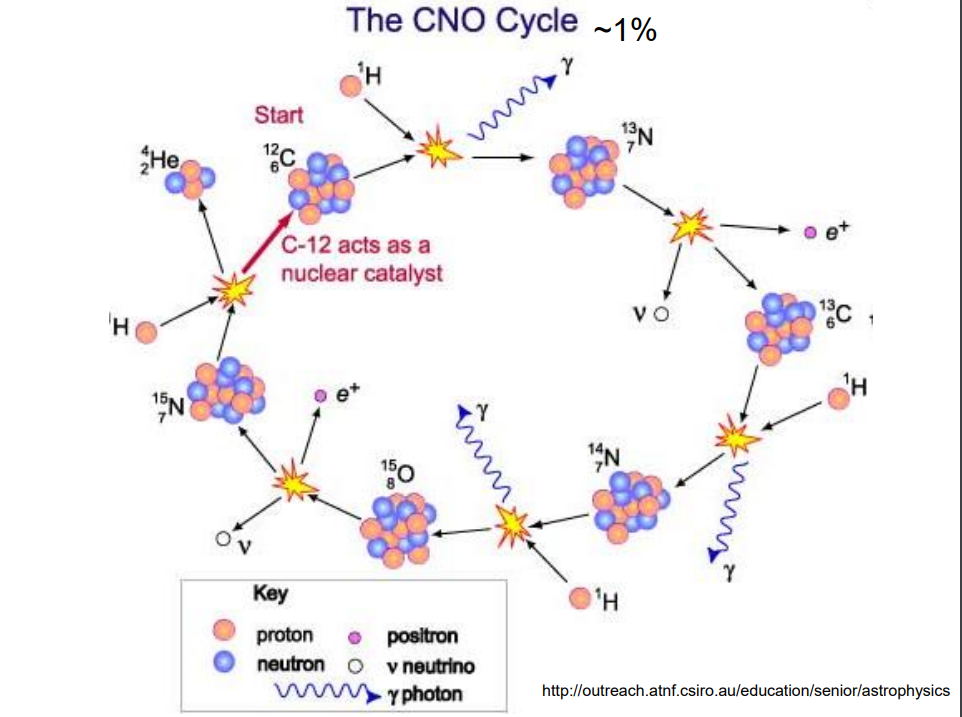
\includegraphics[width=15cm]{images/CNOSynteza.png}
                \end{center}
                Energia wydzielona w reakcjach syntezy unoszona jest przez produkty reakcji i (z wyjątkiem neutrina) przekazywana jest ośrodkowi. Energia zależy od rodzaju reakcji, a dokładniej od wielkości defektu masy. Tempo zachodzenia reakcji zależy od warunków panujących wewnątrz jądra gwiazdy. Poniżej wzory pozwalające je obliczyć:
                \begin{equation}
                    \varepsilon_\text{pp} \approx 120 \autoround{\frac{X_H}{0.5} }^2 \autoround{\frac{\rho}{10^{5}\:m^{-3}}}\autoround{\frac{T}{15\cdot 10^6\:K}}^4\: Wm^{-3}
                \end{equation}
                \begin{equation}
                    \varepsilon_\text{CN} \approx 2\autoround{\frac{X_H}{0.5}}\autoround{\frac{X_{N14}}{0.006} }\autoround{\frac{\rho}{10^5\: m^{-3}} }\autoround{\frac{T}{15\cdot 10^6\:K}}^{16} Wm^{-3}
                \end{equation}
                gdzie \(X_H\) i \(X_{N{14}}\) określają obfitość występowania wodoru i azotu czternaście. W przypadku słońca 99\% energi dostarcza cykl pp a 1\% cykl CNO. Ten stosunek zależy od temperatury:
                \begin{center}
                    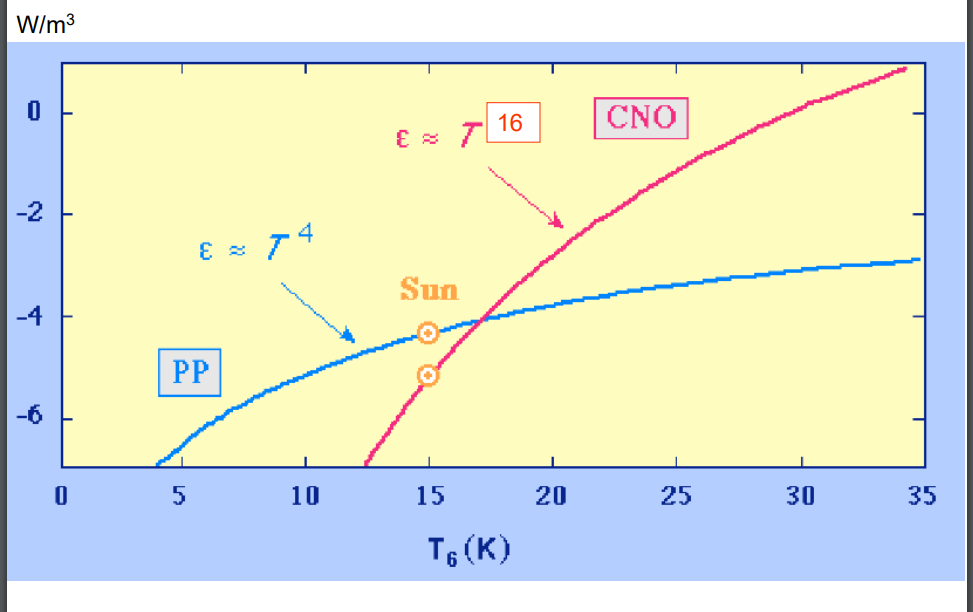
\includegraphics[width=15cm]{images/cykleSynteza.png}
                \end{center}
                Jako że tempo reakcji termojądrowych wpływa na parametry gwiazdy, to w gwiazdach ustala się stan równowagi \--- taki, że produkowana energia może być odprowadzona w takim tempie, żeby nie zmieniać warunków. Jeśli jednak zabraknie gwieździe paliwa, to wówczas żeby móc wykorzystywać inne paliwo zmieniają się warunki panujące w gwieździe (punkt równowagi przesuwa się).\\
                To na ile wystarcza gwieździe paliwa wodorowego określa \textbf{nuklearna skala czasowa}. Dla gwiazd ciągu głównego opisywana jest wzorem:
                \begin{equation}
                    \tau_\text{nuc} \approx 10^{10}\text{lat} \cdot \frac{M}{M_\odot} \cdot \frac{L_\odot}{L} = 10^{10}\text{lat} \cdot \autoround{\frac{M}{M_\odot}}^{-2.8}
                \end{equation}
                Dla słońca ten czas wynosi około 10 miliardów lat. Ze wzoru wynika, że gwiazdy masywne przebywają na ciągu głównym znacznej krócej niż gwiazdy mało masywne (np. czerwone karły).
        \subsection{Transport energii w gwiazdach}
            Transport energii z wnętrza gwiazd na jego powierzchnie może zachodzić na kilka sposobów jednak najważniejsze to \textbf{transport promienisty} i \textbf{konwekcja}.
            \subsubsection{Transport promienisty}
                Za ten rodzaj transportu odpowiedzialne są wielokrotnie pochłaniane i ponownie emitowane fotony. Czas jaki zajmuje fotonowi dotarcie na powierzchnie w przypadku Słońca to kilka milionów lat. Przez ten okres foton jest pochłaniany i emitowany \(\sim 10^{22}\) razy. W rezultacie fotony opuszczające gwiazdę są 4-6 rzędów wielkości mniej energetyczne niż te wyemitowane w wyniku syntezy jądrowej. Przepływ energii traktuje się jako proces dyfuzyjny i korzystając z m. in. \textbf{prawa Ficka}.
            \subsubsection{Konwekcja}
                Konwekcja polega na turbulentnych ruchach materii, konsekwencją których jest odprowadzenie energii z obszaru, w którym jest jej za dużo. Konwekcja, w odróżnieniu od transportu promienistego pozwala odprowadzić dowolnie dużą nadwyżkę energii \--- jest więc głównym mechanizmem transportu energii w gwiazdach, gdy konieczne jest odprowadzenie dużej ilości energii. Konwekcja likwiduje dysproporcje w składzie chemicznym. Jest także odpowiedzialna za zjawisko \textbf{granulacji} \--- widocznych na powierzchni komórek konwekcji odprowadzających energię z wnętrza słońca:
                \begin{center}
                    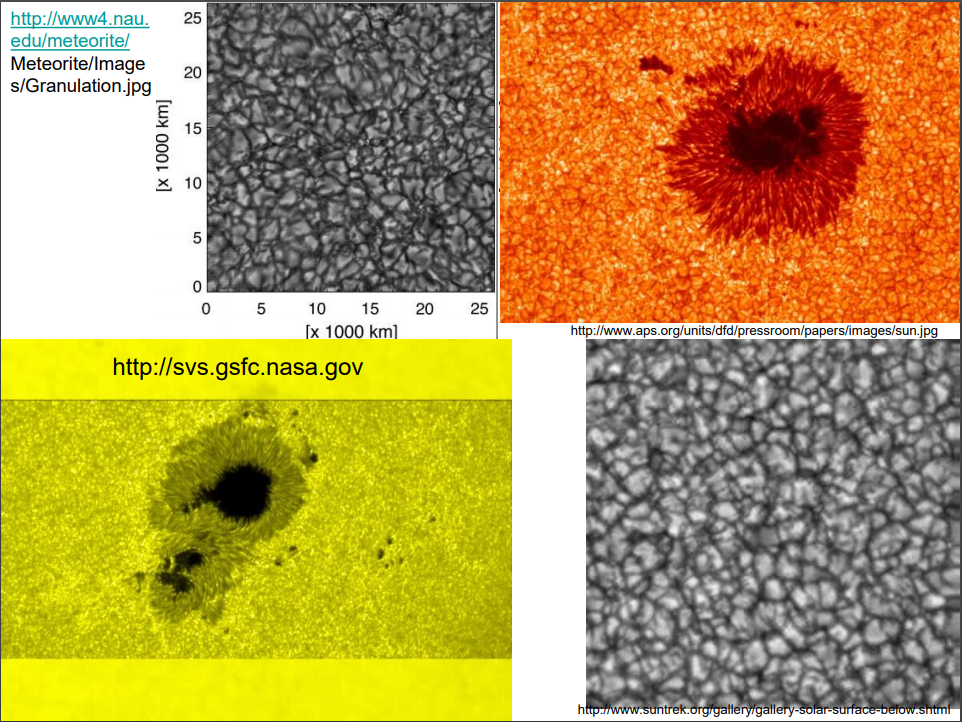
\includegraphics[width=15cm]{images/granule.png}
                \end{center}
\end{document}